% !TEX root = mythesis.tex

%==============================================================================
\chapter{Data Analysis}
\label{sec:data_analysis}
%==============================================================================
\section{Image Visual Inspection}
\section{Surface Brightness Analysis}
\subsection{Full Azimuthal Surface Brightness}
To accurately quantify potential asymmetries in the X-ray emission of NGC 1550, surface brightness analysis is performed. First, the emission center is estimated by constructing a \(2'\) aperture around the apparent center, as given in Section X. This aperture size is chosen to capture a statistically significant number of photons while minimizing bias from potential asymmetries outside the group center. The flux-weighted average of the image coordinates within this aperture yields a right ascension of \SI{64.909}{\degree} and a declination of \SI{2.414}{\degree}. Concentric Anulli with \(1'\) width are constructed from the calculated flux-weighted surface brightness of the group up to \(80'\). The counts \(C\) within each annulus are determined using the \texttt{funcnts} task from the \texttt{funtools} software, with a Poisson error of \(\sqrt{C}\). The surface brightness \(S\) for each annulus is calculated by
\begin{align*}
    S = \frac{C_\text{image} - C_\text{PIB}}{C_\text{expmap}\cdot A},
\end{align*}
where \(C\) denotes the counts in the photon image, total PIB map, and exposure map, respectively. Errors are calculated using Gaussian error propagation. Furthermore, background estimation is performed using \(10\) circular regions with a \(48'\) radius, each centered \(160'\) from the calculated center of NGC 1550. The average background surface brightness is evaluated for all circles combined and separately for the northern (Circles 1-5) and southern region (Circles 6-10) to account for possible background gradients. Table TODO lists the average background for all 3 cases. As is clear from the table, all background values consist with each other within a \(1\sigma\)-Intervall. Thus, for the following analysis and interpretation, the total background value obtained from all circles is utilized. 
\begin{figure}[htbp]
    \centering
    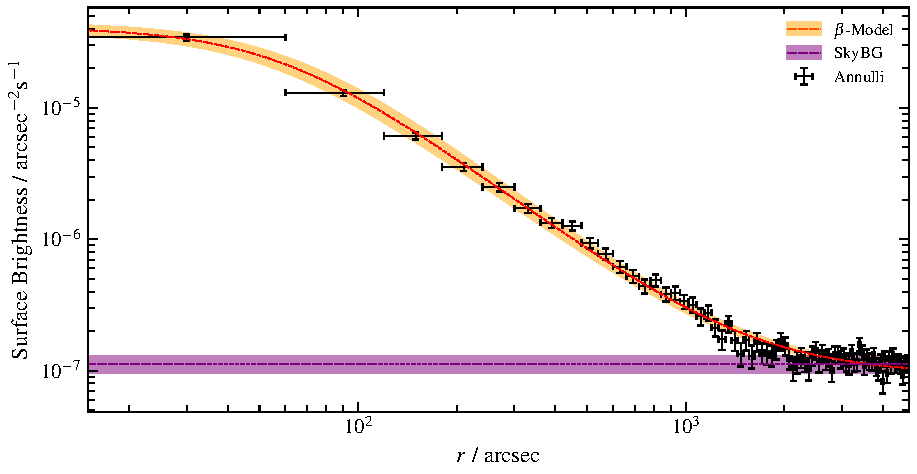
\includegraphics{data_analysis/beta_motel_tot_surf_bri_anulli1_1arcmin.pdf}
    \caption{Surface Brightness within each annulus (black crosses) as a function of distance from the determined SB-center. The dashed orange line represents the best \(\beta\)-model fit, while the purple line indicates the observationally determined background. The shaded regions correspond to their respective \(1\sigma\) intervals.}
    \label{fig:tot_azimuthal_beta_model}
\end{figure}
\begin{table}[h]
    \centering
    \begin{tabular}{lS[table-format=1.2e-1]S[table-format=1.2e-1]}
        \toprule
        Region & {Background} & {Interval} \\
        \midrule
        Southern Background & 13e-08 & 2.0e-09 \\
        Northern Background & 9.9e-08 & 1.2e-08 \\
        Total Background    & 11e-08 & 1.7e-08 \\
        \bottomrule
    \end{tabular}
    \caption{Average background surface brightness for southern, northern, and total regions.}
    \label{tab:background}
\end{table}
A \(\beta\)-Model is employed to characterize the surface brightness profile, given by
\begin{align*}
    S(r) = S_0 \left(1 + \left(\frac{r}{r_c}\right)^2\right)^{-3\beta + 0.5} + d
\end{align*}
where \(d\) represents the background level. The center of each annulus is taken to be \(r\) and the corresponding surface brightness values are utilized. The optimized parameters and \(\chi^2 / \text{d.o.f}\) (Chi squared per degrees of freedom) are listed in Table \ref{table:full_az_fit_parameters}. Figure \ref{fig:tot_azimuthal_beta_model} illustrates the surface brightness as a function of radial distance from the center, including both the fitted \(\beta\)-Model and the observationally estimated background level.
\begin{table}[h!]
    \centering
    \begin{tabular}{lcccc}
    \toprule
    Parameter & $S_0$ & $\beta$ & $r_c$ & $d$ \\
    \midrule
        & $(4.1 \pm 0.4) \times 10^{-5}$ & $0.478 \pm 0.008$ & $60 \pm 5$ & $(9.3 \pm 0.4) \times 10^{-8}$ \\
    \midrule
    \(\chi^2 / \text{d. o. f}\) & \multicolumn{4}{c}{0.96} \\
    \bottomrule
    \end{tabular}
    \caption{Fit parameters, their errors, and the reduced chi-squared value.}
    \label{table:full_az_fit_parameters}
\end{table}
As one can clearly see from \ref{fig:tot_azimuthal_beta_model} and the \(\chi^2/\text{d.o.f}\) value of \(0.96\), the beta model describes the surface brightness profile well and a value of \(\beta = \num{0.478\pm0.008}\) is obtained.
\subsection{Beta Model and Residual Image}
